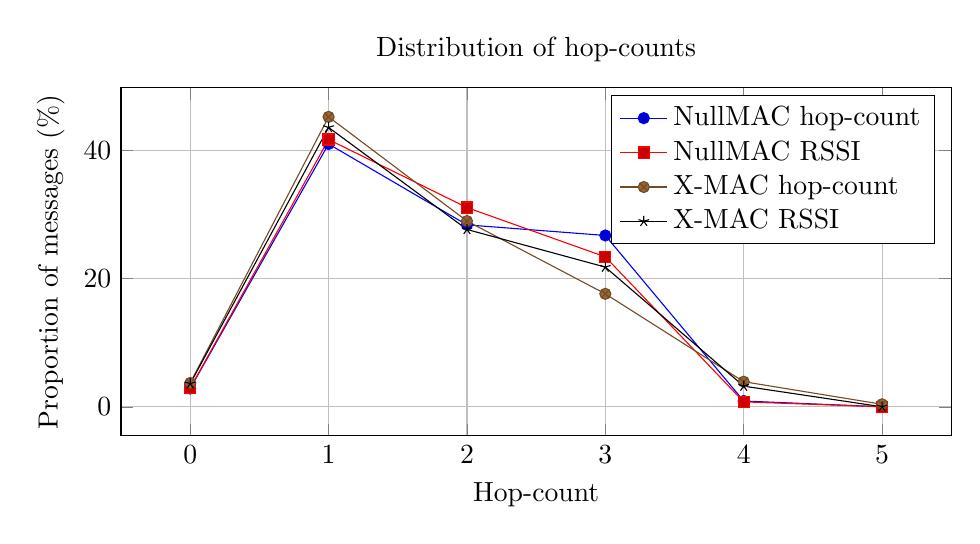
\begin{tikzpicture}
\begin{axis}[
	title=Distribution of hop-counts,
	width=\textwidth,
	height=6cm,
	grid=major,
	ylabel={Proportion of messages (\%)},
	xlabel={Hop-count},
	legend style={
		cells={anchor=west}
	}
]
\addplot coordinates {(0, 2.857142857142857) (1, 41.05263157894737) (2, 28.421052631578947) (3, 26.766917293233083) (4, 0.9022556390977444) (5,0)};
\addplot coordinates {(0, 2.9275808936825885) (1, 41.756548536209553) (2, 31.124807395993837) (3, 23.420647149460708) (4, 0.7704160246533128) (5,0)};
\addplot coordinates {(0, 3.725490196078431) (1, 45.294117647058824) (2, 29.01960784313726) (3, 17.647058823529413) (4, 3.92156862745098) (5, 0.392156862745098)};
\addplot coordinates {(0, 3.6053130929791274) (1, 43.64326375711575) (2, 27.703984819734345) (3, 21.821631878557876) (4, 3.225806451612903) (5,0)};

\legend{NullMAC hop-count, NullMAC RSSI, X-MAC hop-count, X-MAC RSSI}
\end{axis}
\end{tikzpicture}